Eine häufige Problemstellung in der Numerischen Mathematik lautet lineare Gleichungssysteme mit großen, dünn besetzten Matrizen zu lösen.
Dabei kommen meist iterative Verfahren zum Einsatz, die in diesm Projekt effizient implementiert werden.
\subsection*{a)}
Generieren Sie eine symmetrisch positiv definite Zufallsmatrix $A \in \mathbb{R}^{n\times n}$, wobei pro Zeile eine fixe Anzahl an Einträgen
ungleich Null sind. Testen Sie für eine zufällige rechte Seite $b \in \mathbb{R}^n$ bis zu welcher Größe $n$ das lineare
Gleichungssystem
\begin{align*}
  Ax = b
\end{align*}
mit einem direkten Löser (numpy.linalg.solve) in akzeptabler Zeit gelöst werden kann.
Welchen Aufwand erwarten Sie abhängig von n? Plotten Sie die Rechenzeit in Abhängigkeit von der Problemgröße.
\begin{lstlisting}[language=Python]

def zufallsmatrix(n, nonzeros):
	A = np.concatenate((np.zeros((n,nonzeros)), np.random.rand(n, n-nonzeros)), axis = 1)
	for i in range(n):
		np.random.shuffle(A[i])
	return A + A.T + np.diag(np.random.rand(n)*10)

A_base = zufallsmatrix(5000,100)
\end{lstlisting}
\begin{figure}
    \centering
    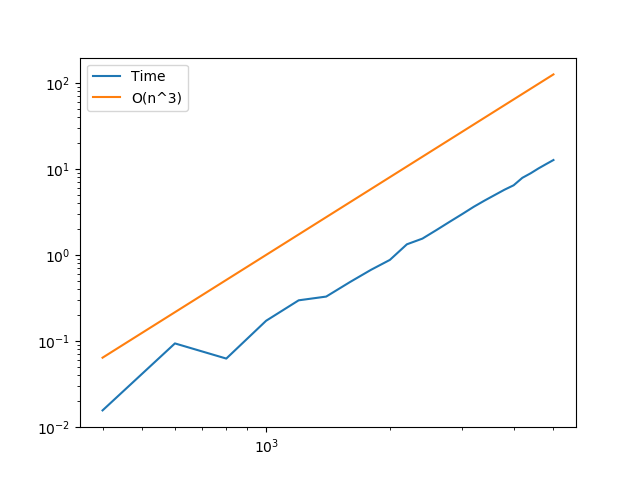
\includegraphics[width=\linewidth]{Aufgabe_1/plot_a.png}
    \caption{Rechenzeit abhängig von der Problemgröße}
    \label{fig:my_label}
\end{figure}
Wie in Abbildung 1 ersichtlich verhält sich die Rechenzeit kubisch in Relation zur Problemgröße.
Zum Testen wurde eine Zufallsmatrix mit 100 Nicht-Null-Einträgen pro Zeile (nicht exakt, da die Symmetriesierung den Wert pro
Zeile verzerrt) und einer Gesamtgröße von 5000 erstellt. Der direkte Löser wurde schließlich auf die $(200k \times 200k)$-dimensionalen Ausschnitte der oberen rechten Ecke angewandt ($2 \leq k \leq 25$). Wie man sieht erreichen wir damit schon langsam die Grenze
des akzeptabel Berechenbaren, für die volle $5000\times5000$-Matrix braucht der Algorithmus schon über 10 Sekunden.
\FloatBarrier
\subsection*{b)}
Implementierung des CG-Verfahrens:
\begin{lstlisting}[language=Python]
def cg(A,b,x0,tol):
    xt = x0
    r0 = b - np.dot(A,xt)
    d = r0
    while(np.linalg.norm(r0) > tol):
        prod = np.dot(np.transpose(r0),r0)
        prod2 = np.dot(A,d)
        alpha = prod/np.dot(np.transpose(d),prod2)
        xt = xt + alpha*d
        r0 = r0 - alpha*prod2
        beta = np.dot(np.transpose(r0),r0)/prod
        d = r0 + beta*d
    return xt
\end{lstlisting} \label{cg}
Wir beweisen die Äquivalenz des obigen Algorithmus zu Algorithmus 8.10 im Numerik-Skript mittels Induktion: \\
Dabei bezeichnen wir mit * die Variablen aus unserem Algorithmus und ohne * die Variablen des Algorithmus
aus dem Skript. \\
Induktionsanfang: \\
\begin{align*}
   &A = A^*, b = b^*, x_0 = x_0^* \\
   &r_0 = b - Ax_o = b^* - A^*x_0^* = r_0^* \\
   &d_0 = r_0 = r_0^* = d_0^* \\
   &\alpha_0 = \frac{r_0^Td_0}{d_0^TAd_0} = \frac{r_0^{*T}d_0^*}{d_0^{*T}Ad_0^*} = \frac{r_0^{*T}r_0^*}{d_0^{*T}Ad_0^*} = \alpha_0^* \\
   &x_1 = x_0 + \alpha_0d_0 = x_0^* + \alpha_0^*d_0^* = x_1^* \\
   &r_1 = b - Ax_1 = b^* - A^*x_1^* = b^* - A^*x_0^* - \alpha_0^*Ad_0^* = r_0^* - \alpha_0^*A^*d_0^* = r_1^* \\
   &\beta_0 = - \frac{r_1^TAd_0}{d_0^TAd_0} = \frac{-r_1^{*T}Ad_0^*}{d_0^{*T}Ad_0^*} = \frac{-r_1^{*T}Ar_0^*}{r_0^{*T}Ar_0^*}
\end{align*}
Unter Ausnutzung der Orthogonalität der Residuen erhalten wir: $r_1^{*T}r_0^* = 0$ und somit können wir den Bruch
folgendermaßen erweitern:
\begin{align*}
  \frac{-r_1^{*T}Ar_0^*}{r_0^{*T}Ar_0^*} = \frac{r_1^{*T}r_0^* -\alpha_0^*r_1^{*T}Ar_0^*}{\alpha_0^*r_0^{*T}Ar_0^*}
\end{align*}
Nun berechen wir
\begin{align*}
  r_1^{*T}r_1^* = r_1^{*T}(r_0^*-\alpha_0^*Ad_0^*) = r_1^{*T}r_0^* - \alpha_0^*r_1^{*T}Ar_0^*
\end{align*}
und setzen $\alpha_0^* = \frac{r_0^{*T}r_0^*}{d_0^{*T}Ad_0^*}$ ein:
\begin{align*}
  \frac{r_1^{*T}r_0^* -\alpha_0^*r_1^{*T}Ar_0^*}{\alpha_0^*r_0^{*T}Ar_0^*} = \frac{r_1^{*T}r_1^*}{\frac{r_0^{*T}r_0^*}{r_0^{*T}Ar_0^*}r_0^{*T}Ar_0^*}
  = \frac{r_1{*T}r_1^*}{r_0^{*T}r_0^*} = \beta_0^* \\
  d_1 = r_1 + \beta_0d_0 = r_1^* + \beta_0^*d_0^* = d_1^*
\end{align*}
Damit haben wir die Gleichheit der Variablen nach dem ersten Schleifendurchlauf gezeigt. \\
Sei nun nach $n$ Schleifendurchläufen die Gleichheit aller vorhergehenden Variablen vorausgesetzt: \\
\begin{align*}
  \alpha_{n-1} = \alpha_{n-1}*, x_n = x_n^*, r_n = r_n^*, \beta_{n-1} = \beta_{n-1}*, d_n = d_n^* \\
  \alpha_n = \frac{r_n^Td_n}{d_n^TAd_n} = \frac{r_n^{*T}d_n^*}{d_n^{*T}A^*d_n^*} = \frac{r_n^{*T}(r_n^* + \beta_{n-1}^*d_{n-1}^*)}{d_n^{*T}A^*d_n^*} \\
\end{align*}
Jetzt nutzen wir die Eigenschaft: $\forall 0 \leq j < m: r_m^Td_j = 0$ und erhalten:
\begin{align*}
  \frac{r_n^{*T}(r_n^* + \beta_{n-1}^*d_{n-1}^*)}{d_n^{*T}A^*d_n^*} = \frac{r_n^{*T}r_n^*}{d_n^{*T}A^*d_n^*} = \alpha_n^* \\
  x_{n+1} = x_n + \alpha_nd_n = x_n^* + \alpha_n^*d_n^* = x_{n+1}^* \\
  r_{n+1} = b - Ax_{n+1} = b - A(x_n + \alpha_nd_n) = b - Ax_n - \alpha_nd_n = \\
  = r_n - \alpha_nAd_n = r_n^* - \alpha_n^*A^*d_n^* = r_{n+1}^* \\
  \beta_n = - \frac{r_{n+1}^TAd_n}{d_n^TAd_n} = \frac{r_{n+1}^{*T}r_n^* - \alpha_n^*r_{n+1}^{*T}A^*d_n^*}{d_n^{*T}A^*d_n^*}
  = \frac{r_{n+1}{*T}r_{n+1}^*}{r_n^{*T}r_n^*} = \beta_n^* \\
  d_{n+1} = r_{n+1} + \beta_nd_n = r_{n+1}^* + \beta_n^*d_n^* = d_{n+1}^*
\end{align*}
Und der Beweis ist vollständig. \\

Rechenschritte pro Schleifendurchlauf: \\
Am aufwändigsten ist natürlich die Matrix-Vektor-Multiplikation, wovon wir in unserem Algorithmus
im Gegensatz zu jenem aus dem Skript nur eine pro Schleifendurchlauf benötigen.
Zusätzlich dazu brauchen wir 3 Vektor-Vektor-Multiplikationen und 4 Vektor-Skalar-Operationen. \\
Damit erhalten wir insgesamt $n^2+7n$ Flops pro Durchlauf. \\
Im Vergleich dazu verwendet der Algorithmus aus dem Numerik-Skript pro Iteration zwei Matrix-Vektor-Multiplikationen
und ist daher aus Effizienzgründen unterlegen. \\

Die Theorie besagt, dass das CG-Verfahren spätentens nach $n$ Durchläufen die exakte Lösung liefert und für die Iterierten
folgende Fehlerabschätzung gilt:
\begin{align*}
  \Vbraces{x^{(t)}-A^{-1}b}_A \leq 2\left(\frac{1-1/\sqrt{\kappa}}{1+1/\sqrt{\kappa}}\right)^t\Vbraces{x^{(0)}-A^{-1}b}_A, \quad t \in \N,
\end{align*}
mit der spektralen Konditionszahl $\kappa = \text{cond}_2(A)$. \\
Also sollte das Verfahren exponentiell kovergieren ($\Landau{AB^t}$) mit Konstanten\\
$A = 2\Vbraces{x^{(0)}-A^{-1}b}_A, \quad B = \frac{1-1/\sqrt{\kappa}}{1+1/\sqrt{\kappa}}$\\
Wie in untenstehender Grafik ersichtlich scheint bei unseren Zufallsmatrizen der Wert von $B$ sich in etwa bei $0.92$ einzupendeln
und unsere vorgegebene Toleranz von $10^{-8}$ wird bereits nach etwa $350$ Iterationen erreicht, noch weit vor dem theoretisch
(bis auf Rechenfehler) garantierten exakten Resultat nach $n = 5000$ Durchläufen.
Ansonsten verhält sich der Fehler wie wir ihn erwarten würden. \\
Unsere Testwerte: \\

\begin{lstlisting}[language=Python]
n = 5000
A = np.random.rand(n,n)
A = np.dot(A,np.transpose(A))
A += 10*np.diag(abs(np.random.random(n)))
b = np.random.rand(n)
tol = 10**(-8)
x0 = np.random.rand(n)*10
\end{lstlisting}

\begin{figure}
    \centering
    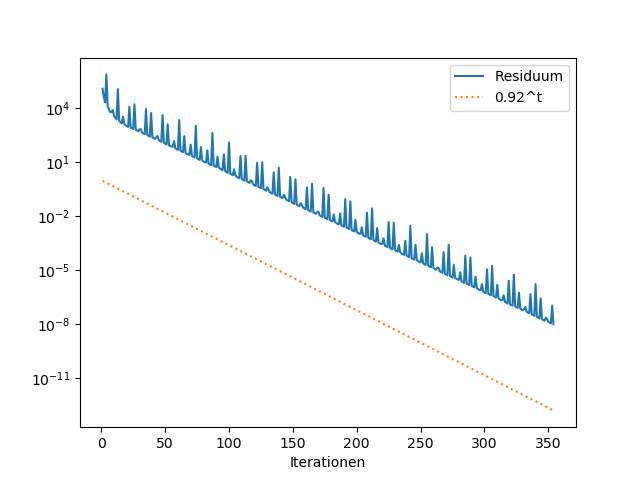
\includegraphics[width=\linewidth]{Aufgabe_1/plot_b.png}
    \caption{Residuum abhängig von der Anzahl an Iterationen}
    \label{fig:my_label}
\end{figure}
\FloatBarrier
\subsection*{c)}
Dünn besetzte Matrizen erlauben effizientere Implementierungen als voll besetzte, indem beim Speichern und Rechnen
nur Einträge die ungleich Null sind berücksichtigt werden. Eine Möglichkeit einer solchen Implementierung ist das sogenannte
\textit{compressed sparse row} Format. Anstelle aller Einträge $A_{ij}, i,j = 1,\dots,n$ einer Matrix $A \in \mathbb{R}^{n\times n}$
werden ein Vektor $v \in \mathbb{R}^{n\times n}$ aller Einträge ungleich Null, ein Vektor $J \in \mathbb{N}_0^m$ von Spaltenindizes
und ein Vektor $I \in \mathbb{N}_0^{n+1}$ von Zeigern gespeichert. Die $i$-te Zeile von $A$ ist dann gegeben durch
\begin{align*}
  A_{ij} = \begin{cases}
    v_{k(j)}, & \text{falls}~ j \in \{J_{I_i}, J_{I_i} + 1, \dots, J_{I_i + 1} - 1\} \\
    0, & \text{sonst}
  \end{cases}
\end{align*}
Implementierung in Python: \\
\begin{lstlisting}[language=Python]
class Sparse:

    def __init__(self,b,v, J = np.zeros(0), I = np.zeros(0)):
        if b:
            self.v = np.array(v)
            self.J = np.array(J)
            self.I = np.array(I)
            self.n = len(self.I)-1
        else:
            self.v, self.J, self.I = self.fromdense(v)
            self.n = len(self.I)-1

    def __matmult__(self,b):
        d = np.zeros(self.n)
        for i in range(self.n):
            x = np.array(self.J[self.I[i]:self.I[i+1]]).astype(int)
            d[i] = self.v[self.I[i]:self.I[i+1]]@b[x]
        return d


    def todense(self):
        A = np.zeros([self.n,self.n])
        for i in range(self.n):
            for j in range(self.I[i],self.I[i+1]):
                A[i][self.J[j]] = self.v[j]
        return A

    def fromdense(self,A):
        v,J = np.zeros(0), np.zeros(0)
        I = np.array([0])
        c = 0
        for i in range(np.shape(A)[0]):
            for j in range((np.shape(A))[0]):
                if A[i][j] != 0:
                    v = np.append(v,A[i][j])
                    J = np.append(J,j)
                    c += 1
            I = np.append(I,c)
        return v, J, I
\end{lstlisting}

Da wir bei diesem Projekt uns nur auf das cg-Verfahren konzentrieren, haben wir nur die Matrix-Vektor Multiplikation für die Klasse Sparse implementiert.

\begin{figure}
    \centering
    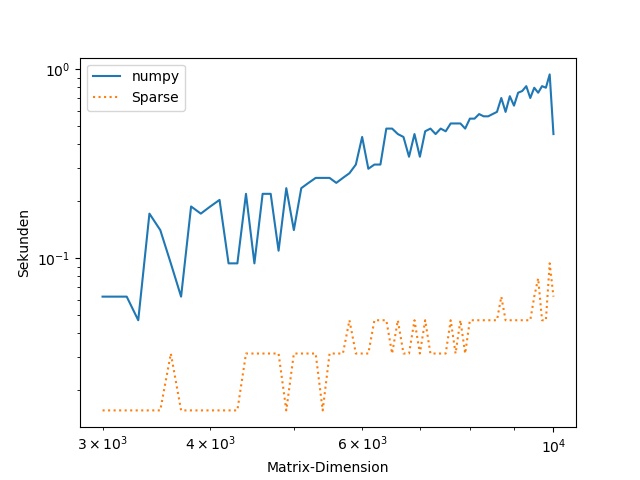
\includegraphics[width=\linewidth]{Aufgabe_1/matmult_plot.png}
    \caption{Vergleich Numpy Matrixmultiplikation vs. Sparse Matrixmultiplikation}
    \label{fig:my_label}
\end{figure}
\FloatBarrier

Hier sehen wir, dass erst ab einer gewissen Größe die Sparse-Multiplikation effizienter gegenüber der Numpy-Multiplikation ist.

\subsection*{d)}
Kombinieren Sie Ihre CG-Implementierung mit Ihrer \textbf{sparse} Klasse und testen Sie die Effizienz: \\
Implementierung:
\begin{lstlisting}[language=Python]
def Scg(A,b,x0,tol):
    xt = x0
    r0 = b - A.__matmult__(xt)
    d = r0
    while(np.linalg.norm(r0) > tol):
        prod = np.dot(np.transpose(r0),r0)
        prod2 = A.__matmult__(d)
        alpha = prod/np.dot(np.transpose(d),prod2)
        xt = xt + alpha*d
        r0 = r0 - alpha*prod2
        beta = np.dot(np.transpose(r0),r0)/prod
        d = r0 + beta*d
    return xt
\end{lstlisting}

Bei dieser CG-Implementierung verwenden wir anstelle der Numpy-Matrix-Vektor-Multiplikation die Implementierung von der Sparse-Klasse.
Zu beachten ist, dass die Matrix A ein Objekt der Klasse Sparse sein muss, damit die Funktion durchgeführt werden kann.
Ansonsten ist die Implementierung ident zum vorherigen cg-Verfahren.

\begin{figure}
    \centering
    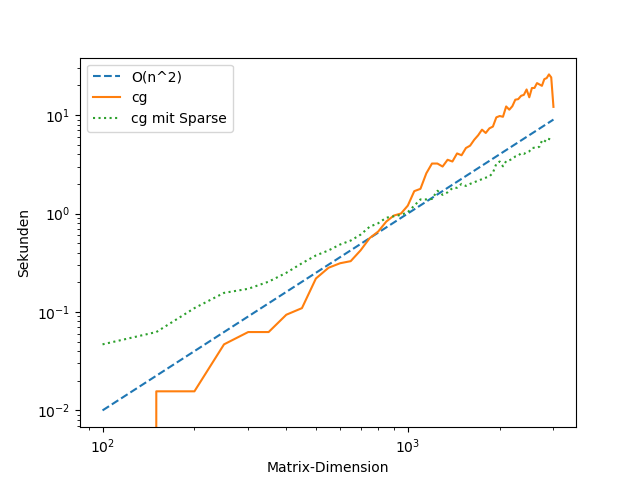
\includegraphics[width=\linewidth]{Aufgabe_1/Cg_Scg.png}
    \caption{cg-Verfahren vs. cg-Verfahren mit Klasse Sparse}
    \label{fig:my_label}
\end{figure}
\FloatBarrier

Ab einer Matrixgröße von ca. 1000 ist das Scg-Verfahren effizienter als die übliche Implementierung.
Man sieht außerdem, dass beide Algorithmen eine Laufzeit von etwa $\Landau{n^2}$
\subsection*{e)}
Die Konvergenzgeschwindigkeit des CG-Verfahrens ist durch die spektrale Konditionszahl cond($A$) der Matrix $A$ bestimmt.
Um die Konvergenzgeschwindigkeit zu erhöhen löst man das vorkonditionierte System
\begin{align*}
  D^{-1}AD^{-1T} = D^{-1}b
\end{align*}
und gewinnt die Lösung $x$ dann durch $x = D^{-1T}y$. Die Matrix $D$ wird dabei so gewählt, dass
\begin{itemize}
\item für beliebige Vektoren $z \in \mathbb{R}^n$ der Vektor $D^{-1T}D^{-1}z$ einfach zu berechen ist und
\item $\text{cond}(D^{-1}AD^{-1T}) < \text{cond}(A)$.
\end{itemize}
Implementierung des vorkonditionierten CG-Verfahrens:
\begin{lstlisting}[language=Python]
    def vcg(A,b,x0,P,tol):
        r0 = b - A.__matmult__(x0)
        P_inv = np.linalg.inv(P)
        z0 = P_inv@r0
        d = z0
        while(np.linalg.norm(r0) > tol):
            prod = np.dot(np.transpose(z0),r0)
            prod2 = A.__matmult__(d)
            alpha = np.dot(np.transpose(r0),z0)/np.dot(np.transpose(d),prod2)
            x0 = x0 + alpha*d
            r0 = r0 - alpha*prod2
            z0 = P_inv@r0
            beta = np.dot(np.transpose(z0),r0)/prod
            d = z0 + beta*d
    return x0
\end{lstlisting}

\subsection*{f)}
Wie in untenstehender Grafik ersichtlich wurde mit der Vorkonditionierung die Anzahl der benötigten Iterationen
zur Erreichung der erwünschten Toleranz exorbitant gesenkt.
\begin{figure}
    \centering
    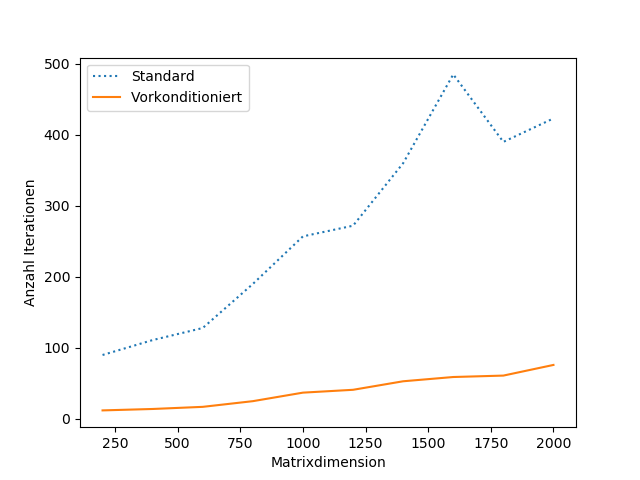
\includegraphics[width=\linewidth]{Aufgabe_1/f.png}
    \caption{Vergleich Anzahl Interationen}
    \label{fig:my_label}
\end{figure}
\begin{figure}
    \centering
    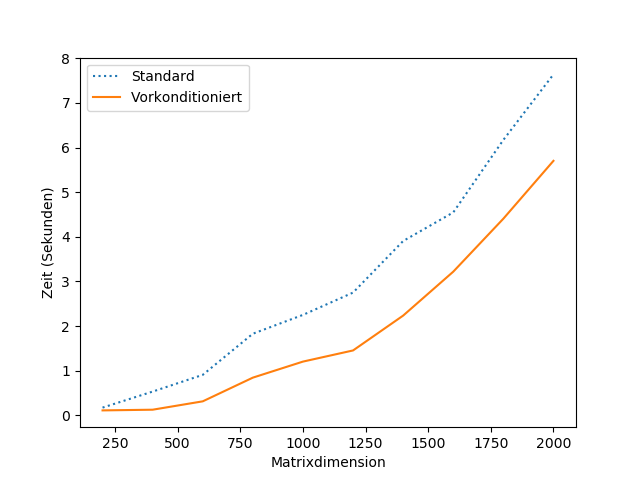
\includegraphics[width=\linewidth]{Aufgabe_1/vcg.png}
    \caption{Vergleich Anzahl Interationen}
    \label{fig:my_label}
\end{figure}
